%%==================================================
%% app1.tex for DUT Thesis
%% version: 0.1
%% last update: Apr 27th, 2022
%%==================================================



\BiChapter{附录内容名称}{Appendix A}
\BiSection{附录内容1}{Appendix A1}
以下内容可放在附录之内:\par
(1) 正文内过于冗长的公式推导;\par
(2) 方便他人阅读所需的辅助性数学工具或表格;\par
(3) 重复性数据和图表;\par
(4) 论文使用的主要符号的意义和单位;\par
(5) 程序说明和程序全文。\par
这部分内容可省略。如果省略,删掉此页。\par
\BiSection{附录内容2}{Appendix A2}

\begin{figure}
	\small
	\centering
	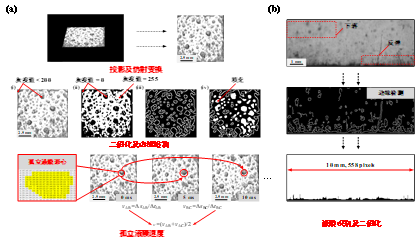
\includegraphics[scale=1.3]{figures/figure6}
	\bicaption{图像处理示意图}{Image processing diagram}\label{fig6:diagram}
\end{figure}
\begin{table}[t]
	\centering
	\bicaption{各参数误差}{Errors E of parameters} \label{}
	\begin{tabular}{m{5em}<{\centering}m{5em}<{\centering}m{5em}<{\centering}}%但由于设置了表格的整体宽度,为了使表格对齐,需要使用表达式 @{\extracolsep{\fill}}
		\toprule[2pt]
		参数 &$E^+$&$E^-$\\
		\midrule[1pt]
		δh/h&	+9.78\%&	−9.78\%\\
		${δA}_{\rm{{wet}}}$/${A}_{\rm{{wet}}}$&	+4.00\%&	0\\
		δd/d	&+2.00\%	&0\\
		δv/v	&+6.58\%&	−6.58\%\\
		Bo	&+19.62\%	&−19.62\%\\
		Ra	&+29.58\%	&−29.58\%\\
		$\rm{{Ma}_{g}}$	&+10.52\%&	−10.52\%\\
		$\rm{Ma}_{R}$	&+6.76\%&	−6.48\%\\
		Wb	&+14.72\%	&−14.59\%\\
		We	&+13.40\% &	−13.25\%\\
		Re	&+7.04\%	&−6.75\%\\	
		Re	&+7.04\%&	−6.75\%\\
		\bottomrule[2pt]
	\end{tabular}
\end{table}